\documentclass[a4paper, 12pt]{article}

\usepackage[portuguese]{babel}
\usepackage[utf8]{inputenc}
\usepackage{amsmath}
\usepackage{indentfirst}
\usepackage{graphicx}
\usepackage{multicol,lipsum}
\usepackage{xcolor}

\usepackage{listings}

\definecolor{verde}{rgb}{0,0.5,0}
\lstset{
  language=C++,
  basicstyle=\ttfamily\small, 
  keywordstyle=\color{blue}, 
  stringstyle=\color{verde}, 
  commentstyle=\color{red}, 
  extendedchars=true, 
  showspaces=false, 
  showstringspaces=false, 
  numbers=left,
  numberstyle=\tiny,
  breaklines=true, 
  backgroundcolor=\color{green!10},
  breakautoindent=true, 
  captionpos=b,
  xleftmargin=0pt,
}

\begin{document}
%\maketitle

\begin{titlepage}
	\begin{center}
	
	%\begin{figure}[!ht]
	%\centering
	%\includegraphics[width=2cm]{c:/ufba.jpg}
	%\end{figure}

		\Huge{Universidade Federal Rural de Pernambuco}\\
		\large{Bacharelado em Ciência da Computação}\\ 
		\vspace{15pt}
        \vspace{95pt}
        \textbf{\LARGE{EP 1 -  Análise de Algorítmos Recursivos e Iterativos}}\\
		%\title{{\large{Título}}}
		\vspace{3,5cm}
	\end{center}
	
	\begin{flushleft}
		\begin{tabbing}
			Aluno: Bruno Henrique Gusmão Vasconcelos \\
			Professor: Rodrigo de Souza \\
	\end{tabbing}
 \end{flushleft}
	\vspace{1cm}
	
	\begin{center}
		\vspace{\fill}
			 Outubro\\
		 2017
			\end{center}
\end{titlepage}
%%%%%%%%%%%%%%%%%%%%%%%%%%%%%%%%%%%%%%%%%%%%%%%%%%%%%%%%%%%

% % % % % % % % %FOLHA DE ROSTO % % % % % % % % % %

\begin{titlepage}
	\begin{center}
	
	%\begin{figure}[!ht]
	%\centering
	%\includegraphics[width=2cm]{c:/ufba.jpg}
	%\end{figure}

		\Huge{Universidade Federal Rural de Pernambuco}\\
		\large{Bacharelado em Ciência da Computação}\\ 
\vspace{15pt}
        
        \vspace{85pt}
        
		\textbf{\LARGE{Relatório}}
		\title{\large{EP 1 -  Análise de Algorítmos Recursivos e Iterativos}}
	%	\large{Modelo\\
     %   		Validação do modelo clássico}
			
	\end{center}
\vspace{1,5cm}
	
	\begin{flushright}

   \begin{list}{}{
      \setlength{\leftmargin}{4.5cm}
      \setlength{\rightmargin}{0cm}
      \setlength{\labelwidth}{0pt}
      \setlength{\labelsep}{\leftmargin}}

      \item Primeiro Relatório de Algoritmos e Estruturas de Dados do Curso de Ciência da Computação ofertado pela Universidade Federal Rural de Pernambuco.

      \begin{list}{}{
      \setlength{\leftmargin}{0cm}
      \setlength{\rightmargin}{0cm}
      \setlength{\labelwidth}{0pt}
      \setlength{\labelsep}{\leftmargin}}

			\item Aluno: Bruno Henrique Gusmão Vasconcelos \
            \item Professor: Rodrigo de Souza \

      \end{list}
   \end{list}
\end{flushright}
\vspace{1cm}
\begin{center}
		\vspace{\fill}
		 Outubro\\
		 2017
			\end{center}
\end{titlepage}
\newpage
% % % % % % % % % % % % % % % % % % % % % % % % % %
\newpage
\tableofcontents
\thispagestyle{empty}

\newpage
\pagenumbering{arabic}
% % % % % % % % % % % % % % % % % % % % % % % % % % %
\section{Resumo}

Este relatório tem como objetivo analisar algoritmos recursivos implementados e compará-los com suas versões iterativas através da quantidade de operações executadas, ou seja, utilizando método experimental para obtenção de resultados.\\

\newpage

\section{Descrição de atividades}

Para obtenção de resultados, utilizaremos algoritmos recursivos e suas versões iterativas, escritos na linguagem C e compilados com o compilador TDM-GCC 4.9.2 64-bit da IDE Dev-C++, e faremos uma comparação entre o número de operações realizadas entre estes algoritmos. \\
Os algoritmos utilizados na análise foram:
\begin{itemize}
	\item MAX-REC  e MAX-IT, sendo o primeiro um algoritmo recursivo do tipo divisão-e-conquista e o segundo sua versão iterativa, para encontrar o valor máximo de um vetor de inteiros.
	\item CRESC-REC e CREC-IT, sendo o primeiro um algoritmo recursivo do tipo divisão-e-conquista e o segundo sua versão iterativa, para ordenar um vetor de forma crescente.
	\item LOC-REC e LOC-IT, sendo o primeiro um algoritmo recursivo do tipo divisão-e-conquista e o segundo sua versão iterativa, para encontrar a posição de um inteiro x em um vetor crescente de inteiros.
	\item SEG-REC e SEG-IT, sendo o primeiro um algoritmo recursivo do tipo divisão-e-conquista e o segundo sua versão iterativa, para calcular o segmento de soma máxima de um vetor de inteiros.
\end{itemize}

\newpage
\section{Análise dos Resultados}

\subsection{MAX-REC}

O algoritmo MAX-REC tem como objetivo encontrar o valor máximo de um vetor de inteiros de forma recursiva, utilizando divisão-e-conquista.\\


Código:

\begin{lstlisting}
int max_rec(int* A, int p, int r)
{
	if(p == r)
	{
		COUNT++;
		return A[p];
	}
	else
	{
		int result, x, y;
		int q = (p + r) / 2;
		
		x =  max_rec(A, p, q);
		COUNT++;
		y = max_rec(A, q+1 , r);
		COUNT++;
		
		result = max( x , y );
			
		return result;		
	}
}
\end{lstlisting}

O algoritmo MAX-REC divide o vetor em dois segmentos repetidamente até que sobre um segmento de um ou dois valores, a partir disso ele retorna para a chamada anterior o maior valor local, tomando dois a dois, até que a primeira função retorne o maior valor absoluto. 

Abaixo podemos observar o gráfico de complexidade deste algoritmo e concluir que ele possui um crescimento linear $n$.

\begin{figure}[h]
	\centering
	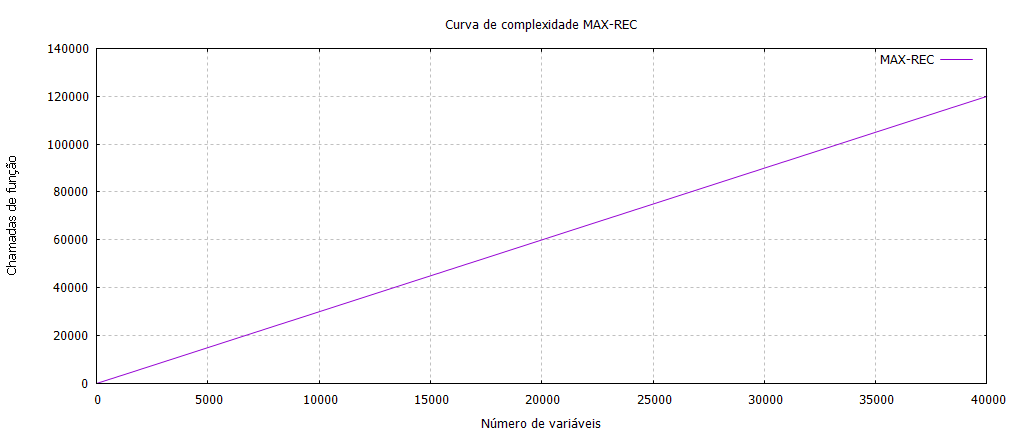
\includegraphics[width=\textwidth]{Algoritmos/graficos/plot-max-rec.png}
	\caption{Curva de complexidade MAX-REC}
	\label{fig:max-rec}
\end{figure}

\newpage
\subsection{MAX-IT}

O algoritmo MAX-IT tem como objetivo encontrar o valor máximo de um vetor de inteiros de forma iterativa.\\


Código:

\begin{lstlisting}
int max_it(int* A, int tamA){
	int i;
	int max = A[0];

	for(i = 0 ; i < tamA ; i++)
	{
		COUNT++;
		if(A[i] > max)
		{
			COUNT++;
			max = A[i];
		}
	}

	return max;	
}
\end{lstlisting}

O algoritmo MAX-IT percorre todo o vetor uma única vez e compara o valor do índice atual com o valor máximo até aquele momento, se o valor do índice atual for maior que o máximo até então, o valor máximo recebe o valor do índice atual até que percorra todo o vetor.


Abaixo podemos observar o gráfico de complexidade deste algoritmo e concluir que ele possui um crescimento linear $n$.

\begin{figure}[h]
	\centering
	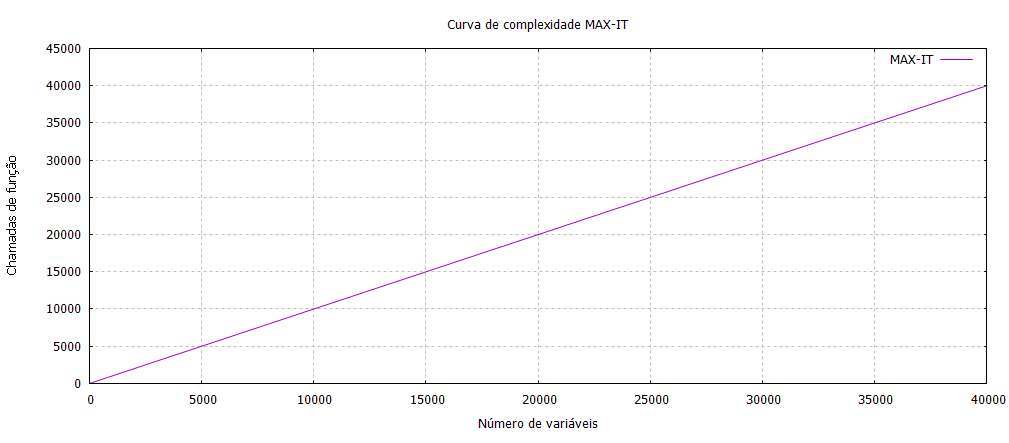
\includegraphics[width=\textwidth]{Algoritmos/graficos/plot-max-it.png}
	\caption{Curva de complexidade MAX-IT}
	\label{fig:max-it}
\end{figure}

\newpage

\subsection{CRESC-REC}

O algoritmo CRESC-REC tem como objetivo ordenar um vetor de inteiros de forma recursiva, utilizando divisao-e-conquista.\\


Código:

\begin{lstlisting}
void cresc_rec(int* arr, int l, int r)
{
    if (l < r)
    {
        int m = l+(r-l)/2;
 
        cresc_rec(arr, l, m);
        COUNT++;
        cresc_rec(arr, m+1, r);
        COUNT++;
 		
        merge(arr, l, m, r);
        COUNT++;
    }
}

void merge(int* arr, int l, int m, int r)
{
    int i, j, k;
    int n1 = m - l + 1;
    int n2 =  r - m;
 
    int L[n1], R[n2]; 

    for (i = 0; i < n1; i++)
        L[i] = arr[l + i];
    for (j = 0; j < n2; j++)
        R[j] = arr[m + 1+ j];
 
    i = 0; 
    j = 0; 
    k = l;
    while (i < n1 && j < n2)
    {
        if (L[i] <= R[j])
        {
            arr[k] = L[i];
            i++;
        }
        else
        {
            arr[k] = R[j];
            j++;
        }
        k++;
    }

    while (i < n1)
    {
        arr[k] = L[i];
        i++;
        k++;
    }
 
    while (j < n2)
    {
        arr[k] = R[j];
        j++;
        k++;
    }
}
\end{lstlisting}

O algoritmo CRESC-REC divide o vetor em dois segmentos repetidamente até que sobre um segmento de um ou dois valores, a partir disso ele chama a função $merge$ que é a continuação da função de forma encapsulada, ela tem como objetivo criar dois subarrays e ordená-los entre si, como o vetor foi destrinchado em segmentos de um ou dois valores, essa função ordena localmente dois a dois até que chegue de volta na primeira chamada da função e retorne a ordenação absoluta.

Abaixo podemos observar o gráfico de complexidade deste algoritmo e concluir que ele possui um crescimento linear $n$.

\begin{figure}[h]
	\centering
	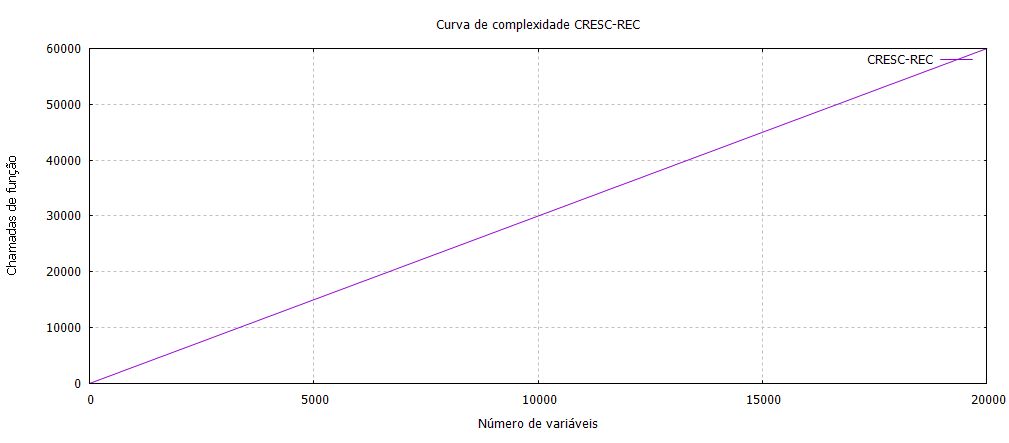
\includegraphics[width=\textwidth]{Algoritmos/graficos/plot-cresc-rec.png}
	\caption{Curva de complexidade CRESC-REC}
	\label{fig:cresc-rec}
\end{figure}

\newpage 


\subsection{CRESC-IT}

O algoritmo CRESC-IT tem como objetivo ordenar um vetor de inteiros de forma iterativa.\\


Código:

\begin{lstlisting}
void cresc_it(int* A, int p, int n)
{
	int i, j, aux;
	for(j = 0 ; j <= n ; j++)
	{
		COUNT++;
		for(i = 1 ; i <= n ; i++)
		{	
			COUNT++;
			if(A[i] < A[i-1])
			{
				aux = A[i];
				A[i] = A[i-1];
				A[i-1] = aux;
			}
		}	
	}
}
\end{lstlisting}

O algoritmo CRESC-IT percorre todo o vetor comparando o valor do índice atual com o valor do índice anterior, se o valor do índice atual for menor que o anterior eles trocam de posição, esse processo é repetido o número de vezes igual ao número de variáveis de entrada.


Abaixo podemos observar o gráfico de complexidade deste algoritmo e concluir que ele possui um crescimento $n^2$.

\begin{figure}[h]
	\centering
	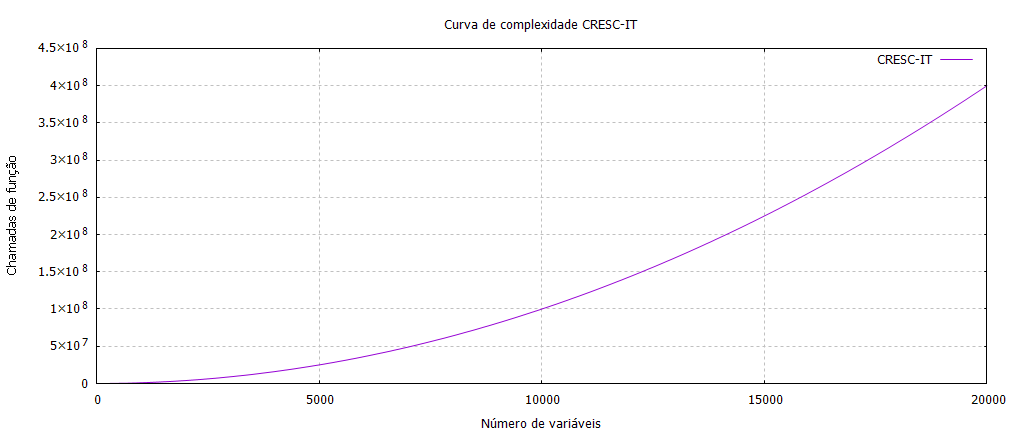
\includegraphics[width=\textwidth]{Algoritmos/graficos/plot-cresc-it.png}
	\caption{Curva de complexidade CRESC-IT}
	\label{fig:cresc-it}
\end{figure}

\newpage

\subsection{LOC-REC}

O algoritmo LOC-REC tem como objetivo encontrar um valor $x$ em um vetor de inteiros ordenado de forma recursiva, utilizando divisão-e-conquista.\\


Código:

\begin{lstlisting}

int loc_rec(int* a, int p, int r, int x)
{
	if(p == r-1)
	{
		COUNT++;
		return r;
	}
	else
	{
		int q = (p + r) / 2; 
		if(a[q] < x)
		{
			COUNT++;
			return loc_rec(a, q, r, x);
		}
		else
		{
			COUNT++;
			return loc_rec(a, p, q, x); 
		}
	}
}	
\end{lstlisting}

O algoritmo LOC-REC divide o vetor em dois segmentos e analisa se o valor procurado é menor ou maior que o valor da metade do segmento, se o valor for maior ele repete o processo a partir da metade do segmento, se for menor ele repete o processo até a metade do segmento. Este processo é repetido até que o valor intermediário seja o procurado. 

Abaixo podemos observar o gráfico de complexidade deste algoritmo e concluir que ele possui um crescimento $nlog(n)$.

\begin{figure}[h]
	\centering
	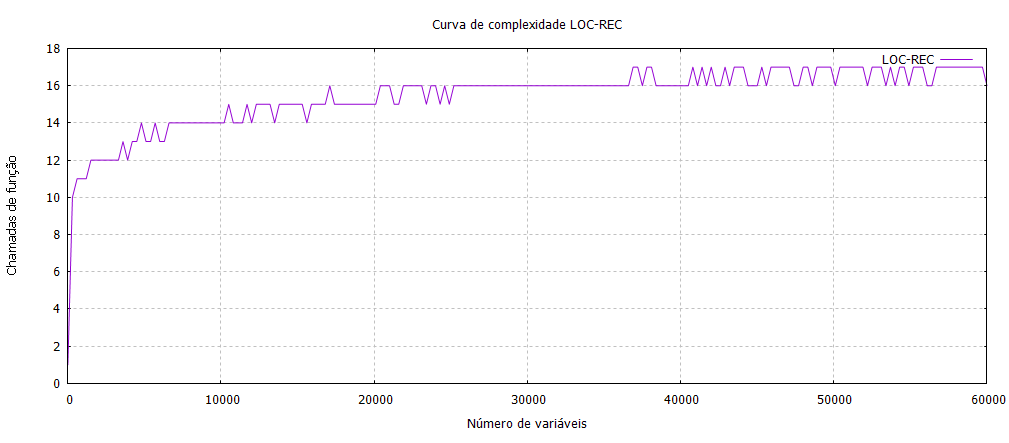
\includegraphics[width=\textwidth]{Algoritmos/graficos/plot-loc-rec.png}
	\caption{Curva de complexidade LOC-REC}
	\label{fig:loc-rec}
\end{figure}

\newpage

\subsection{LOC-IT}


O algoritmo LOC-IT tem como objetivo encontrar um valor $x$ em um vetor de inteiros ordenado de forma iterativa.\\


Código:

\begin{lstlisting}
int loc_it(int* a, int n, int x)
{
	int p = 0;
	int r = n - 1;
	while(p < r - 1)
	{
		COUNT++;
		int q = (p + r) / 2;
		if(a[q] < x)
		{
			p = q;
		}
		else
		{
			r = q;
		}
	}
	return r;
}
\end{lstlisting}

O algoritmo LOC-IT divide o índice máximo por 2 e analisa se o valor procurado é menor ou maior que o intermediário do segmento, se o valor for maior ele repete o processo a partir da metade do segmento, se for menor ele repete o processo até a metade do segmento. Este processo é repetido até que o valor intermediário seja o procurado. 

Abaixo podemos observar o gráfico de complexidade deste algoritmo e concluir que ele possui um crescimento $nlog(n)$.

\begin{figure}[h]
	\centering
	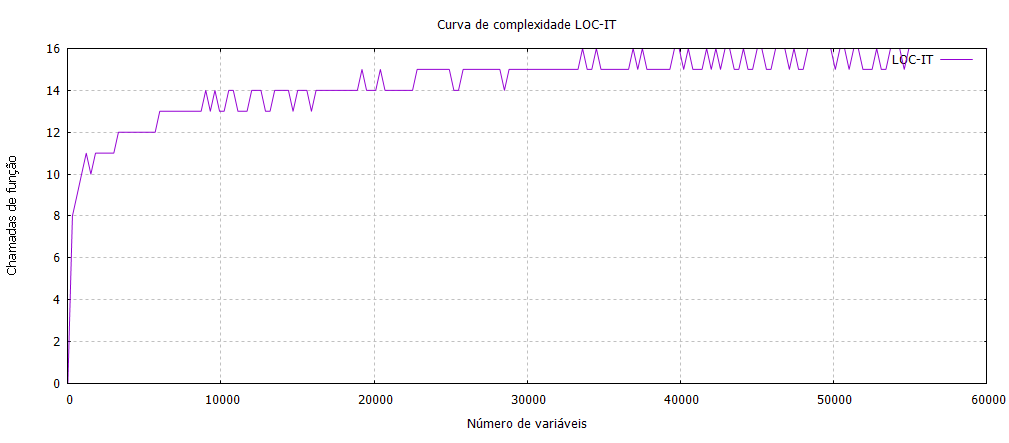
\includegraphics[width=\textwidth]{Algoritmos/graficos/plot-loc-it.png}
	\caption{Curva de complexidade LOC-IT}
	\label{fig:loc-it}
\end{figure}

\newpage

\subsection{SEG-REC}

O algoritmo SEG-REC tem como objetivo encontrar o segmento de soma máxima de um vetor de inteiros de forma recursiva, utilizando divisão-e-conquista.\\


Código:

\begin{lstlisting}
int seg_rec(int* a, int p, int r)
{
	if(p == r)
	{
		return a[p];
	}
	else
	{
		int x1, x2;
		int q = (p + r) / 2;
		
		x1 = seg_rec(a, p, q);
		COUNT++;
		
		x2 = seg_rec(a, q+1, r);
		COUNT++;
		
		int s = a[q];
		int y1 = s;
		int i;
		for(i = q - 1 ; i > p ; i--)
		{
			s += a[i];
			if(s > y1)
			{
				y1 = s;
			}
		}
		s = a[q+1];
		int y2 = s;
		int j;
		for(j = q + 2 ; j < r ; j++)
		{
			s += a[j];
			if(s > y2)
			{
				y2 = s;
			}
		}
		int x = max(max(x1 , y1 + y2), x2);
		return x;
	}
}
\end{lstlisting}

O algoritmo SEG-REC divide o vetor em dois segmentos repetidamente até que sobre um valor e o armazena, a cada retorno da função ele verifica se a soma com o próximo valor é maior que a anterior, se sim ele continua retornando os valores até obter o maior segmento.

Abaixo podemos observar o gráfico de complexidade deste algoritmo e concluir que ele possui um comportamento $f(n) = n$.

\begin{figure}[h]
	\centering
	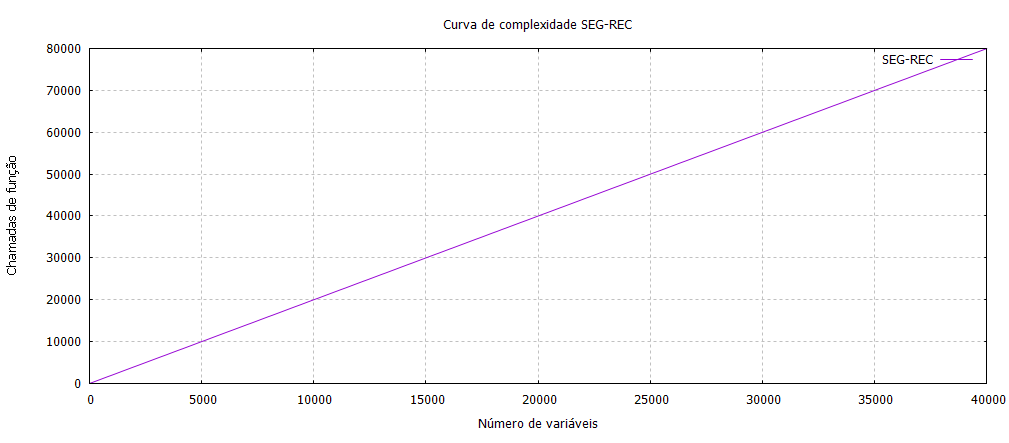
\includegraphics[width=\textwidth]{Algoritmos/graficos/plot-seg-rec.png}
	\caption{Curva de complexidade SEG-REC}
	\label{fig:seg-rec}
\end{figure}

\newpage


\subsection{SEG-IT}


O algoritmo SEG-IT tem como objetivo encontrar o segmento de soma máxima de um vetor de inteiros de forma iterativa.\\


Código:

\begin{lstlisting}
int seg_it(int* a, int p, int r)
{
	int x = a[r];	
	int q;
	int s;
	int j;
	for(q = r - 1 ; q >= p ; q--)	
	{
		COUNT++;
		s = 0;
		for(j = q ; j <= r ; j++)
		{
			COUNT++;
			s = s + a[j];
			if(s > x)				
			{
				x = s;	
			}
		}
	}
	return x;
}
\end{lstlisting}

O algoritmo SEG-IT percorre o vetor verificando os elementos um a um, depois verifica a soma dois a dois, depois a soma três a três até verificar a soma do vetor inteiro e retorna o maior segmento de soma calculado.  

Abaixo podemos observar o gráfico de complexidade deste algoritmo e concluir que ele possui um comportamento $n^2$.

\begin{figure}[h]
	\centering
	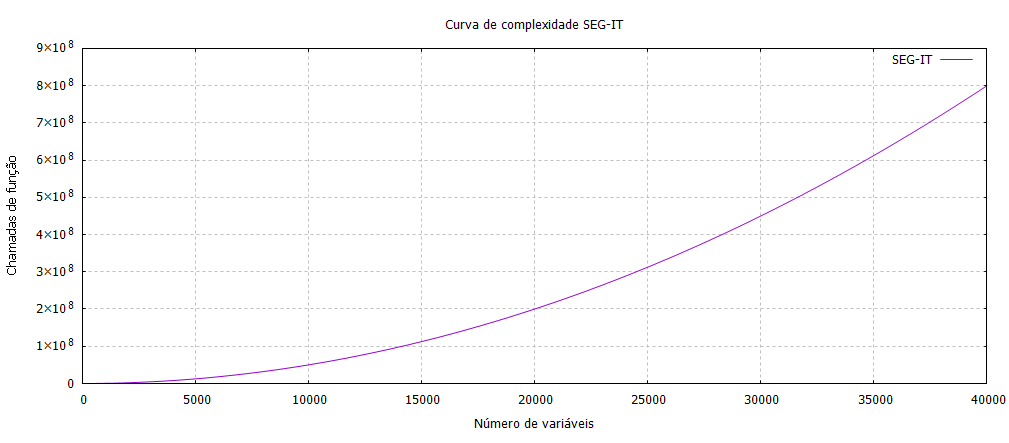
\includegraphics[width=\textwidth]{Algoritmos/graficos/plot-seg-it.png}
	\caption{Curva de complexidade SEG-IT}
	\label{fig:seg-it}
\end{figure}

\newpage

\subsection{Comparações}

Podemos comparar os gráficos de crescimento de cada algoritmo recursivo com sua versão iterativa e tirar conclusões sobre suas complexidades e eficiências.

\newpage

\subsubsection{MAX}

\begin{figure}[h]
	\centering
	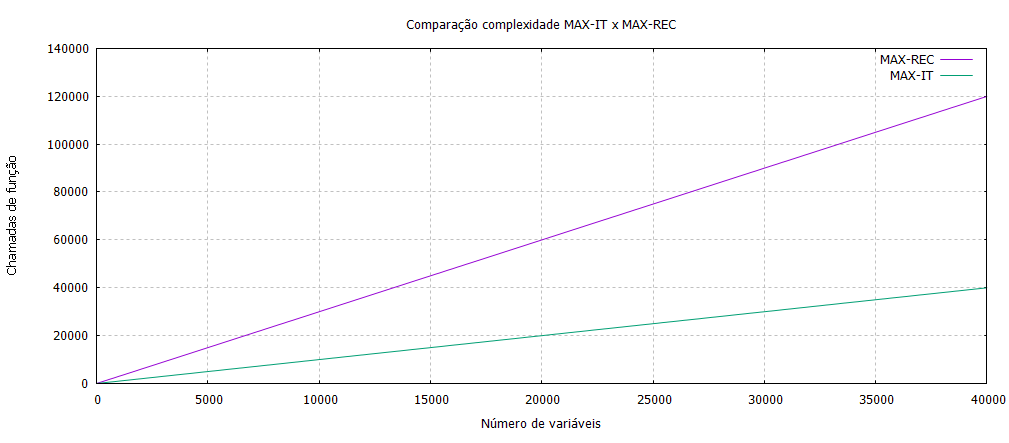
\includegraphics[width=\textwidth]{Algoritmos/graficos/plot-comp-max.png}
	\caption{Comparação de complexidade MAX-REC x MAX-IT}
	\label{fig:max}
\end{figure}

Pelo gráfico traçado podemos observar que o algoritmo iterativo tem menor ângulo de inclinação, resultando numa maior eficiência.

Porém, se formos analisar a complexidade de forma grosseira, eles obedecem a mesma regra de complexidade $n$. O que é facilmente contornável com um processamento mais potente.

\newpage
\subsubsection{CRESC}

\begin{figure}[h]
	\centering
	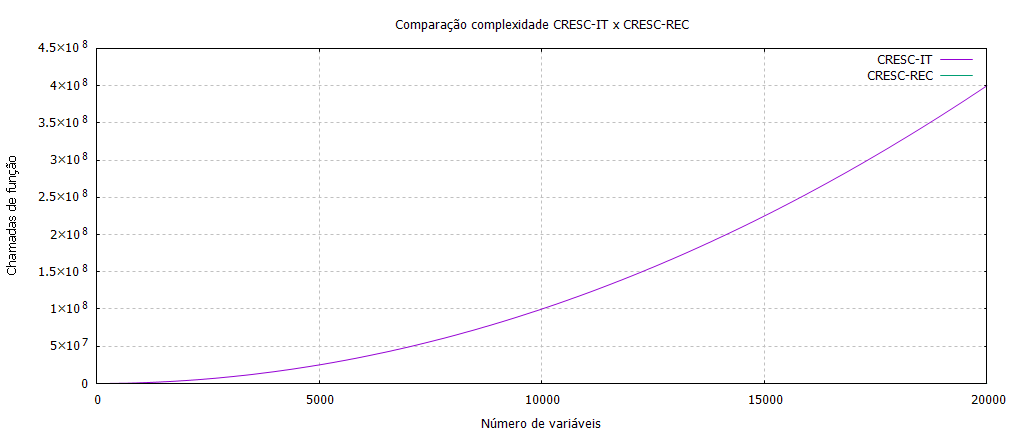
\includegraphics[width=\textwidth]{Algoritmos/graficos/plot-comp-cresc.png}
	\caption{Comparação de complexidade CRESC-REC x CRESC-IT}
	\label{fig:cresc}
\end{figure}

Na comparação dos algoritmos CRESC-REC para CRESC-IT já podemos ver uma significante diferença. Olhando para o gráfico, quase não conseguimos observar o traço de CRESC-REC por ele ter uma complexidade $n$, enquanto o CRESC-REC possui complexidade $n^2$. Isso mostra que, neste caso, a solução recursiva é muito mais eficiente que a iterativa.

\newpage
\subsubsection{LOC}

\begin{figure}[h]
	\centering
	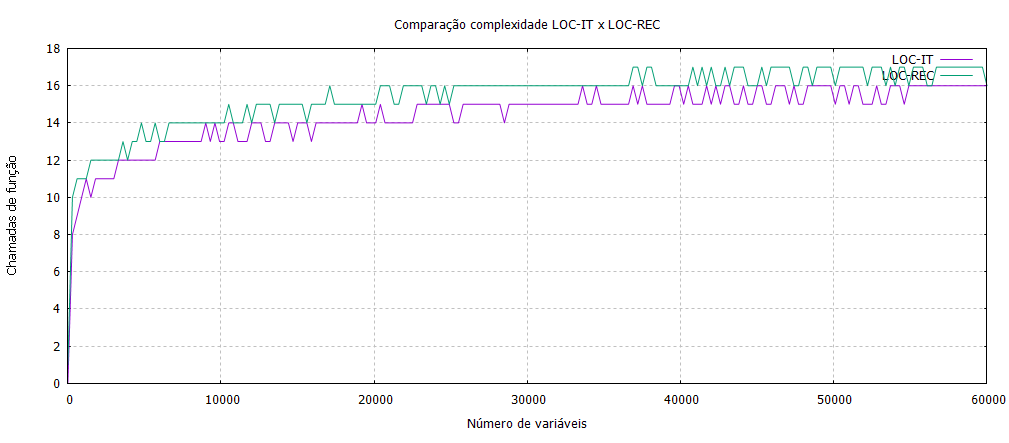
\includegraphics[width=\textwidth]{Algoritmos/graficos/plot-comp-loc.png}
	\caption{Comparação de complexidade LOC-REC x LOC-IT}
	\label{fig:loc}
\end{figure}

Quando comparamos o gráfico dos algoritmos LOC-REC e LOC-IT, podemos ver que eles acompanham basicamente a mesma curva de complexidade $nlog(n)$, logo, são igualmente eficientes.
	
\newpage

\subsubsection{SEG}

\begin{figure}[h]
	\centering
	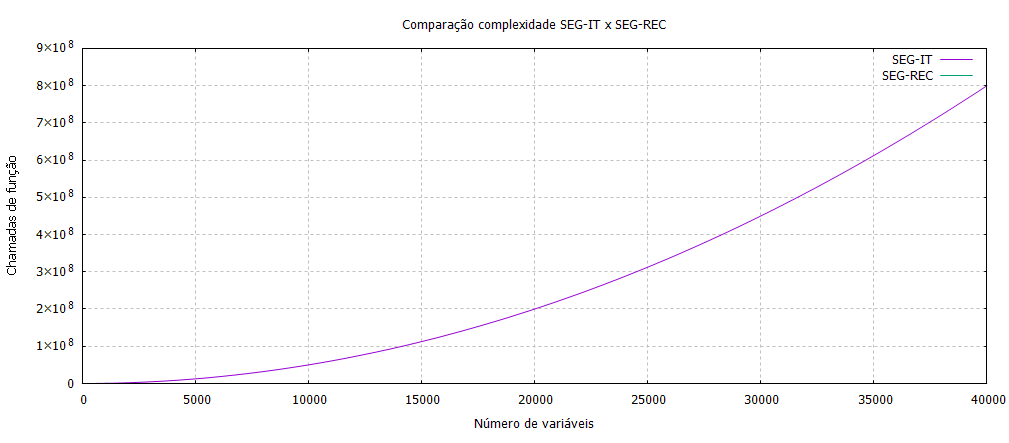
\includegraphics[width=\textwidth]{Algoritmos/graficos/plot-comp-seg.png}
	\caption{Comparação de complexidade SEG-REC x SEG-IT}
	\label{fig:seg}
\end{figure}

Na comparação dos gráficos dos algoritmos SEG-REC e SEG-IT, assim como os algoritmos de ordenação CRESC, vemos que a curva de complexidade da forma iterativa cresce muito mais que a recursiva. Isso se dá porque o número de chamadas SEG-REC tem complexidade $n$, enquanto a SEG-IT possui complexidade $n^2$.


\newpage

\section{Conclusão}

Pela observação dos dados obtidos e aspectos analisados podemos concluir que embora a solução recursiva não tenha sido a melhor em cem porcento dos casos, a facilidade de contornar uma situação é muito maior que um algoritmo iterativo, pois sua eficiência diferencia em apenas uma constante. Já nos casos onde a solução recursiva foi melhor, pudemos observar que a curva de complexidade diferenciava significantemente em relação ao modo iterativo, sendo muito difícil contornar a situação através de melhoria de processamento, tendo a necessidade de recorrer a um algoritmo mais eficiente.

\newpage

\addcontentsline{toc}{section}{Bibliografia}
\section*{Bibliografia}
\footnotesize{

\noindent{Referências Bibliográficas nas Normas ABNT de Livros e Sites (links) – Como Fazer. Disponível em: $<https://www.normaseregras.com/normas-abnt/referencias>$. Acesso em: 29 out. 2017.}\\ \\
\noindent{WILLIAMS, T.; KELLEY, C. gnuplot 5.0, An Interactive Plotting Program. Disponível em: $<http://www.gnuplot.info/docs_5.0/gnuplot.pdf>$. Acesso em: 23 out. 2017.}\\ \\
\noindent{FEOFILOFF, Paulo. Minicurso de Análise de Algoritmos. Disponível em: $<https://www.ime.usp.br/~pf/livrinho-AA/AA-BOOKLET.pdf>$.}\\ \\
\noindent{Merge Sort. Disponível em: $<http://www.geeksforgeeks.org/merge-sort/>$. Acesso em: 18 out. 2017.}

}
\end{document}

